\documentclass{article}

\usepackage{arxiv}

\usepackage[utf8]{inputenc} % allow utf-8 input
\usepackage[T1]{fontenc}    % use 8-bit T1 fonts
\usepackage{lmodern}        % https://github.com/rstudio/rticles/issues/343
\usepackage{hyperref}       % hyperlinks
\usepackage{url}            % simple URL typesetting
\usepackage{booktabs}       % professional-quality tables
\usepackage{amsfonts}       % blackboard math symbols
\usepackage{nicefrac}       % compact symbols for 1/2, etc.
\usepackage{microtype}      % microtypography
\usepackage{graphicx}

\title{The Explainability of Time Series Downsampling}

\author{
    Morgan Frodsham
   \\
    School of Computing \\
    Newcastle University \\
  Newcastle upon Tyne, UK \\
  \texttt{\href{mailto:M.C.M.Frodsham2@newcastle.ac.uk}{\nolinkurl{M.C.M.Frodsham2@newcastle.ac.uk}}} \\
   \And
    Matthew Forshaw
   \\
    School of Computing \\
    Newcastle University \\
  Newcastle upon Tyne, UK \\
  \texttt{\href{mailto:matthew.forshaw@newcastle.ac.uk}{\nolinkurl{matthew.forshaw@newcastle.ac.uk}}} \\
  }

% Pandoc syntax highlighting
\usepackage{color}
\usepackage{fancyvrb}
\newcommand{\VerbBar}{|}
\newcommand{\VERB}{\Verb[commandchars=\\\{\}]}
\DefineVerbatimEnvironment{Highlighting}{Verbatim}{commandchars=\\\{\}}
% Add ',fontsize=\small' for more characters per line
\usepackage{framed}
\definecolor{shadecolor}{RGB}{248,248,248}
\newenvironment{Shaded}{\begin{snugshade}}{\end{snugshade}}
\newcommand{\AlertTok}[1]{\textcolor[rgb]{0.94,0.16,0.16}{#1}}
\newcommand{\AnnotationTok}[1]{\textcolor[rgb]{0.56,0.35,0.01}{\textbf{\textit{#1}}}}
\newcommand{\AttributeTok}[1]{\textcolor[rgb]{0.13,0.29,0.53}{#1}}
\newcommand{\BaseNTok}[1]{\textcolor[rgb]{0.00,0.00,0.81}{#1}}
\newcommand{\BuiltInTok}[1]{#1}
\newcommand{\CharTok}[1]{\textcolor[rgb]{0.31,0.60,0.02}{#1}}
\newcommand{\CommentTok}[1]{\textcolor[rgb]{0.56,0.35,0.01}{\textit{#1}}}
\newcommand{\CommentVarTok}[1]{\textcolor[rgb]{0.56,0.35,0.01}{\textbf{\textit{#1}}}}
\newcommand{\ConstantTok}[1]{\textcolor[rgb]{0.56,0.35,0.01}{#1}}
\newcommand{\ControlFlowTok}[1]{\textcolor[rgb]{0.13,0.29,0.53}{\textbf{#1}}}
\newcommand{\DataTypeTok}[1]{\textcolor[rgb]{0.13,0.29,0.53}{#1}}
\newcommand{\DecValTok}[1]{\textcolor[rgb]{0.00,0.00,0.81}{#1}}
\newcommand{\DocumentationTok}[1]{\textcolor[rgb]{0.56,0.35,0.01}{\textbf{\textit{#1}}}}
\newcommand{\ErrorTok}[1]{\textcolor[rgb]{0.64,0.00,0.00}{\textbf{#1}}}
\newcommand{\ExtensionTok}[1]{#1}
\newcommand{\FloatTok}[1]{\textcolor[rgb]{0.00,0.00,0.81}{#1}}
\newcommand{\FunctionTok}[1]{\textcolor[rgb]{0.13,0.29,0.53}{\textbf{#1}}}
\newcommand{\ImportTok}[1]{#1}
\newcommand{\InformationTok}[1]{\textcolor[rgb]{0.56,0.35,0.01}{\textbf{\textit{#1}}}}
\newcommand{\KeywordTok}[1]{\textcolor[rgb]{0.13,0.29,0.53}{\textbf{#1}}}
\newcommand{\NormalTok}[1]{#1}
\newcommand{\OperatorTok}[1]{\textcolor[rgb]{0.81,0.36,0.00}{\textbf{#1}}}
\newcommand{\OtherTok}[1]{\textcolor[rgb]{0.56,0.35,0.01}{#1}}
\newcommand{\PreprocessorTok}[1]{\textcolor[rgb]{0.56,0.35,0.01}{\textit{#1}}}
\newcommand{\RegionMarkerTok}[1]{#1}
\newcommand{\SpecialCharTok}[1]{\textcolor[rgb]{0.81,0.36,0.00}{\textbf{#1}}}
\newcommand{\SpecialStringTok}[1]{\textcolor[rgb]{0.31,0.60,0.02}{#1}}
\newcommand{\StringTok}[1]{\textcolor[rgb]{0.31,0.60,0.02}{#1}}
\newcommand{\VariableTok}[1]{\textcolor[rgb]{0.00,0.00,0.00}{#1}}
\newcommand{\VerbatimStringTok}[1]{\textcolor[rgb]{0.31,0.60,0.02}{#1}}
\newcommand{\WarningTok}[1]{\textcolor[rgb]{0.56,0.35,0.01}{\textbf{\textit{#1}}}}

% tightlist command for lists without linebreak
\providecommand{\tightlist}{%
  \setlength{\itemsep}{0pt}\setlength{\parskip}{0pt}}

% From pandoc table feature
\usepackage{longtable,booktabs,array}
\usepackage{calc} % for calculating minipage widths
% Correct order of tables after \paragraph or \subparagraph
\usepackage{etoolbox}
\makeatletter
\patchcmd\longtable{\par}{\if@noskipsec\mbox{}\fi\par}{}{}
\makeatother
% Allow footnotes in longtable head/foot
\IfFileExists{footnotehyper.sty}{\usepackage{footnotehyper}}{\usepackage{footnote}}
\makesavenoteenv{longtable}

% Pandoc citation processing
\newlength{\cslhangindent}
\setlength{\cslhangindent}{1.5em}
\newlength{\csllabelwidth}
\setlength{\csllabelwidth}{3em}
\newlength{\cslentryspacingunit} % times entry-spacing
\setlength{\cslentryspacingunit}{\parskip}
% for Pandoc 2.8 to 2.10.1
\newenvironment{cslreferences}%
  {}%
  {\par}
% For Pandoc 2.11+
\newenvironment{CSLReferences}[2] % #1 hanging-ident, #2 entry spacing
 {% don't indent paragraphs
  \setlength{\parindent}{0pt}
  % turn on hanging indent if param 1 is 1
  \ifodd #1
  \let\oldpar\par
  \def\par{\hangindent=\cslhangindent\oldpar}
  \fi
  % set entry spacing
  \setlength{\parskip}{#2\cslentryspacingunit}
 }%
 {}
\usepackage{calc}
\newcommand{\CSLBlock}[1]{#1\hfill\break}
\newcommand{\CSLLeftMargin}[1]{\parbox[t]{\csllabelwidth}{#1}}
\newcommand{\CSLRightInline}[1]{\parbox[t]{\linewidth - \csllabelwidth}{#1}\break}
\newcommand{\CSLIndent}[1]{\hspace{\cslhangindent}#1}

\begin{document}
\maketitle


\begin{abstract}
Enter the text of your abstract here.
\end{abstract}

\keywords{
    blah
   \and
    blee
   \and
    bloo
   \and
    these are optional and can be removed
  }

\hypertarget{introduction}{%
\section{INTRODUCTION}\label{introduction}}

HM Government is committed to making data-driven decisions that engender
public trust
\protect\hyperlink{ref-data2017}{{[}1{]}}--\protect\hyperlink{ref-data2022}{{[}4{]}}.
Data-driven decisions are considered to be ``more well-informed''
\protect\hyperlink{ref-data2017}{{[}1{]}}, effective
\protect\hyperlink{ref-data2022}{{[}4{]}}, consistent
\protect\hyperlink{ref-data2021}{{[}3{]}}, and better ``at scale''
\protect\hyperlink{ref-data2020}{{[}2{]}}. Despite this, there is a lack
of trust in government use of data
\protect\hyperlink{ref-trust}{{[}5{]}}. This suggests that public trust
in data-driven decisions goes beyond how the ``data complies with legal,
regulatory and ethical obligations''
\protect\hyperlink{ref-data2021}{{[}3{]}}. The UK public need to have
``confidence and trust in how data, including personal data, is used''
\protect\hyperlink{ref-data2020}{{[}2{]}}, and this requires
transparency \protect\hyperlink{ref-trust}{{[}5{]}}.

To make data-driven decisions, government decision-makers also need to
trust how the data used (cite user research here). This means trusting
which data points are selected, how this data collected and stored, and
the capability of data practitioners to understand the quality, insights
and limitations of it. At every stage of the data processing pipeline,
data practitioners have the opportunity to communicate the impact of the
assumptions and choices they are making to support decision-makers in
trusting the data informing their decisions.

Time series data is used across HM Government
\protect\hyperlink{ref-pathway}{{[}6{]}} to inform decision-makers
across various domains \protect\hyperlink{ref-onstool}{{[}7{]}}. It is
also widely generated and used by industry and research
\protect\hyperlink{ref-TVStore}{{[}8{]}}. The volume of time series data
is continuously increasingly \protect\hyperlink{ref-datapoint}{{[}9{]}},
posing significant challenges for handling and visualising this popular
data type \protect\hyperlink{ref-TVStore}{{[}8{]}}. Data practitioners
must utilise methods that reduce data volumes to align with limitations
like processing time, computing costs, storage capabilities, and
sustainability ambitions \protect\hyperlink{ref-TVStore}{{[}8{]}},
\protect\hyperlink{ref-Sveinn}{{[}10{]}},
\protect\hyperlink{ref-Shift}{{[}11{]}}.

Downsampling is an established technique
\protect\hyperlink{ref-downsampling}{{[}12{]}},
\protect\hyperlink{ref-sampling}{{[}13{]}} that involves selecting a
representative subset of data to preserve its original shape while
reducing the number of data points
\protect\hyperlink{ref-datapoint}{{[}9{]}},
\protect\hyperlink{ref-MinMaxLTTB}{{[}14{]}}. This is a vital part of
making voluminous time series understandable for human observation
\protect\hyperlink{ref-Sveinn}{{[}10{]}} and an essential step in many
time series database solutions
\protect\hyperlink{ref-datapoint}{{[}9{]}}. However, little attention
has been devoted to how downsampling impacts decision-makers trust in
the data.

Despite widespread use, how to communicate the impact of downsampling
algorithms on time series data remains also understudied
\protect\hyperlink{ref-datapoint}{{[}9{]}},
\protect\hyperlink{ref-Sveinn}{{[}10{]}}. Downsampling expands the
boundaries of risk for decision-makers as data practitioners may not
realise the significance of the data being discarded. Such choices
throughout the data pipeline may have disproportionately larger
consequences later as their ramifications for future decisions are not
fully understood by all. It is important, therefore, that data
practitioners are able to communicate the impact of choices made
throughout the data pipeline.

To address these challenges, this paper shares initial insights from
user research on the impact of downsampling on decision-makers' trust in
data and suggests a visualisation methodology for communicating the
impact of downsampling algorithms on time series. This methodology
combines user research with R packages \texttt{imputeTS}
\protect\hyperlink{ref-imputeTS_R}{{[}15{]}} and \texttt{Rcatch22}
\protect\hyperlink{ref-catch22_R}{{[}16{]}} to identify and visualise
time series features that are most sensitive to downsampling. It is
hoped this will improve decision-makers' trust in data by helping data
practitioners to create transparency in the data processing pipeline,
communicate the impact of downsampling, and support conversations about
which algorithms or parameters are most appropriate for particular
decision-maker use cases.

\hypertarget{related-work}{%
\section{RELATED WORK}\label{related-work}}

\label{sec:headings}

This section provides an overview of previous related work to create a
clear understanding of the most relevant fields of research and identify
the gaps being addressed by the paper.

\textbf{2.1 Data Transparency}

Technology transparency, ``including institutional data practices'', is
sociopolitical in nature
\protect\hyperlink{ref-political_transparency}{{[}17{]}}. There is a
growing number of researchers reflecting on ``societal needs in terms of
what is made transparent, for whom, how, when and in what ways, and,
crucially, who decides''
\protect\hyperlink{ref-social_transparency}{{[}18{]}}.

The implicit assumption behind calls for transparency is that ``seeing a
phenomenon creates opportunities and obligations to make it accountable
and thus to change it''
\protect\hyperlink{ref-transparency_lack}{{[}19{]}}. However, without
sufficient agency to explore the information being shared, seeing a
phenomenon often results in ``information overload''
\protect\hyperlink{ref-digital_transparency}{{[}20{]}} that obfuscates
or diverts \protect\hyperlink{ref-transparency_obfuscation}{{[}21{]}}.
Without agency, transparency is increasingly considered to be a fallacy
\protect\hyperlink{ref-transparency_fallacy}{{[}22{]}}.

Meaningful transparency is only realised when the information is
provided with the tools to turn ``access to agency''
\protect\hyperlink{ref-transparency_lack}{{[}19{]}},
\protect\hyperlink{ref-transparency_fallacy}{{[}22{]}}. This suggests
that data practitioners communicating the assumptions and choices made
throughout the data processing pipeline with decision-makers is not
likely to create trust in how the data is used. Instead, data
practitioners should be encouraged to find tools, such as interactive
visualisations \protect\hyperlink{ref-datapoint}{{[}9{]}}, that put
agency into the hands of decision-makers.

\textbf{2.2 Time series visualisation}

Time series data is commonly visualised as a line graph
\protect\hyperlink{ref-Sveinn}{{[}10{]}},
\protect\hyperlink{ref-timenotes}{{[}23{]}}. Line graphs help the human
eye to observe only the most important data points
\protect\hyperlink{ref-Sveinn}{{[}10{]}} by convey the overall shape and
complexity of the time series data
\protect\hyperlink{ref-datapoint}{{[}9{]}},
\protect\hyperlink{ref-downsampling}{{[}12{]}}. The most effective time
series visualisations are, however, interactive
\protect\hyperlink{ref-timenotes}{{[}23{]}},
\protect\hyperlink{ref-plotly}{{[}24{]}}, turning access into agency
\protect\hyperlink{ref-transparency_fallacy}{{[}22{]}} by allowing the
user to access details on demand. Evaluation of time series
visualisation is, therefore, a growing field of research
\protect\hyperlink{ref-timenotes}{{[}23{]}}.

However, this growing field of research does not extend to
visualisations of choices and assumptions made during data processing
pipline. Indeed, such visualisations are a side effect of the research.
This dynamic is exemplified by the R package \texttt{imputeTS}
\protect\hyperlink{ref-imputeTS_R}{{[}15{]}} where the impact of
imputation choices made by the user is only visualised to support the
user through the complete process of replacing missing values in time
series \protect\hyperlink{ref-imputeTS}{{[}25{]}}. The research set out
in this paper harnesses the capabilities of \texttt{imputeTS} and its
`process' visualisations to help data practitioners communicate the
impact of downsampling choices made in the data processing pipeline.

\textbf{2.3 Value Preserving Data Aggregation}

Technological innovation has generated unprecedented amount of time
series data and this data continues to grow
\protect\hyperlink{ref-data2020}{{[}2{]}},
\protect\hyperlink{ref-TVStore}{{[}8{]}},
\protect\hyperlink{ref-storage}{{[}26{]}},
\protect\hyperlink{ref-CatchUp}{{[}27{]}}. For example, tackling climate
change is the UK Government's ``number one international priority''
\protect\hyperlink{ref-IR}{{[}28{]}}, yet climate simulations that help
inform decision-makers generate tens of terabytes per second
\protect\hyperlink{ref-TVStore}{{[}8{]}},
\protect\hyperlink{ref-climate}{{[}29{]}}. Downsampling (value
preserving data aggregation) plays an important role in addressing how
this voluminous data is processed, stored
\protect\hyperlink{ref-TVStore}{{[}8{]}} and visualised
\protect\hyperlink{ref-Sveinn}{{[}10{]}},
\protect\hyperlink{ref-dashql}{{[}30{]}} by minimising computing
resources needed \protect\hyperlink{ref-TVStore}{{[}8{]}}, reducing
network latency, and improving rendering time
\protect\hyperlink{ref-datapoint}{{[}9{]}},
\protect\hyperlink{ref-MinMaxLTTB}{{[}14{]}}.

An overview of commonly used downsampling (value preserving data
aggregation) algorithms is provided in the table below:

\begin{longtable}[]{@{}
  >{\raggedright\arraybackslash}p{(\columnwidth - 2\tabcolsep) * \real{0.1590}}
  >{\raggedright\arraybackslash}p{(\columnwidth - 2\tabcolsep) * \real{0.8410}}@{}}
\caption{Downsampling Algorithms}\tabularnewline
\toprule\noalign{}
\begin{minipage}[b]{\linewidth}\raggedright
Algorithm
\end{minipage} & \begin{minipage}[b]{\linewidth}\raggedright
Description
\end{minipage} \\
\midrule\noalign{}
\endfirsthead
\toprule\noalign{}
\begin{minipage}[b]{\linewidth}\raggedright
Algorithm
\end{minipage} & \begin{minipage}[b]{\linewidth}\raggedright
Description
\end{minipage} \\
\midrule\noalign{}
\endhead
\bottomrule\noalign{}
\endlastfoot
EveryNth & Selects every nth datapoint for downsampling. \\
Percentage Change & TBC \\
Mode-Median Bucket & Finds mode or median within equally sized data
buckets for selection. \\
Min-Std-Error-Bucket & Uses standard error of the estimate (SEE) in
linear regression for downsampling. \\
MinMax & Preserves minimum and maximum of data buckets. \\
OM\textsuperscript{3} & Maintains the minimum and maximum values at
every time interval for rasterizing. \\
M4 & Combines EveryNth and MinMax, selecting the first and last values
of each data bucket as well as the minimum and maximum values. \\
Longest-Line Bucket & Calculates line length (Euclidean distance)
instead of standard error between buckets. \\
Largest-Triangle One-Bucket & All the data points are ranked by
calculating their effective areas. One point with the highest rank
(largest effective area) is selected to represent each bucket. \\
Largest Triangle Three Buckets & The data point that forms the largest
triangular surface between the previously selected data point and the
average value of the next data bucket. \\
MinMaxLTTB & Preselects data using MinMax before applying Largest
Triangle Three Buckets. \\
\end{longtable}

\protect\hyperlink{ref-M4}{{[}32{]}}

Data practitioners have made recent advances in the performance and
evaluation of downsampling approaches
\protect\hyperlink{ref-datapoint}{{[}9{]}},
\protect\hyperlink{ref-downsampling}{{[}12{]}}--\protect\hyperlink{ref-MinMaxLTTB}{{[}14{]}},
\protect\hyperlink{ref-plotly}{{[}24{]}},
\protect\hyperlink{ref-dashql}{{[}30{]}},
\protect\hyperlink{ref-EveryNth}{{[}31{]}},
\protect\hyperlink{ref-MinMaxOrdered}{{[}33{]}}. These advances focus on
the effectiveness of the algorithm in delivering downsampled data that
represents the original data as accurately as possible. This is vital
part of enabling and improving data-driven decision-making, but is
focused on supporting data practitioners in their analysis of the data.
Instead, the research set out in this paper aims to support data
practitioners to communicate the impact of their downsampling choices
for decision-makers.

\textbf{2.4 Time series feature analysis}

The increasing size of modern time series data sets has also generated
new research into the dynamical characteristics of time series
\protect\hyperlink{ref-catch22}{{[}34{]}}. These characteristics are
often used to identify features that enable efficient clustering and
classification of time series data, especially for machine learning. A
comprehensive library of such features is the \emph{hctsa} (highly
comparative time series analysis) toolbox. This shares the 4791 best
performing features after computationally comparing thousands of
features from across scientific time series analysis literature
\protect\hyperlink{ref-fulcher2017}{{[}35{]}}.

Utilising such a library, however, is computationally expensive
\protect\hyperlink{ref-catch22}{{[}34{]}}. C. H. Lubba et. al have
attempted to address this by identified a subset of 22 features that are
tailored to time series data mining tasks
\protect\hyperlink{ref-catch22}{{[}34{]}},
\protect\hyperlink{ref-bagnall}{{[}36{]}}. Although further research is
needed to evaluate the relative performance of different feature sets on
different types of problems, \texttt{catch22} performs well against
other feature libraries across 800 diverse real-world and
model-generated time series \protect\hyperlink{ref-henderson}{{[}37{]}}.

Features used to classify time series data could provide a common
framework by which to consistently compare different downsampling
algorithms and parameters. The research set out in this paper utilises
the \texttt{Rcatch22} subset of features to explore impact of
downsampling and create a visual tool for explaining this impact.

\hypertarget{motivation}{%
\section{MOTIVATION}\label{motivation}}

\label{sec:headings}

\begin{itemize}
\tightlist
\item
  user research insights
\end{itemize}

\hypertarget{methodology}{%
\section{METHODOLOGY}\label{methodology}}

\label{sec:headings}

\textbf{4.1 Data}

The research outlined by this report starts with the eight demonstrative
time series shared by the Alan Turing Institute
\texttt{Annotated\ Change} GitHub repository
\protect\hyperlink{ref-ATIChangePoint}{{[}38{]}}. The demonstrative time
series are synthetic with known change points that provide examples of
different types of time series. These synthetic time series (demo\_100,
demo\_200, demo\_300, demo\_400, demo\_500, demo\_600, demo\_700,
demo\_800) support change point annotators annotate real-world data sets
for the \texttt{Turing\ Change\ Point\ Dataset}
\protect\hyperlink{ref-ATIChangePoint}{{[}38{]}}. Nine synthetic time
series are used for this research as the eighth
\texttt{Annotated\ Change} demonstrative time series (demo\_800) is
multivate and split in two (800A and 800B) for this research to enable
better comparison.

\textbf{4.2 Downsampling}

These nine synthetic time series are imported into \texttt{RStudio} from
JSON scripts and two downsampling algorithms are applied to all with
the\texttt{Jettison\ MVP\ Code}
\protect\hyperlink{ref-Jettison}{{[}39{]}}. These simple algorithms are
chosen to provide initial insights into the impacts of downsampling with
minimally complex code; the algorithm \emph{EveryNth} selects every
other data point and \emph{Percentage Change} selects every data point
that has greater than one per cent difference between the last
transmitted and newest values.

{[}SHOULD I ADD AN EQUATION HERE FOR THE ALGORITHMS?{]}

\[
\xi _{ij}(t)=P(x_{t}=i,x_{t+1}=j|y,v,w;\theta)= {\frac {\alpha _{i}(t)a^{w_t}_{ij}\beta _{j}(t+1)b^{v_{t+1}}_{j}(y_{t+1})}{\sum _{i=1}^{N} \sum _{j=1}^{N} \alpha _{i}(t)a^{w_t}_{ij}\beta _{j}(t+1)b^{v_{t+1}}_{j}(y_{t+1})}}
\] These algorithms are applied iteratively across each time series,
creating parameters 1 to 50 for each downsampling algorithm and
\texttt{Annotated\ Change} time series. There are now 900 time series
for investigation; 450 for each downsampling algorithm.

The R package \texttt{imputeTS}
\protect\hyperlink{ref-imputeTS_R}{{[}15{]}} is applied to the time
series to obtain the data volume, number of missing values (NAs) and
number of gaps. This is important to understand the effect of each
downsampling algorithm across the 900 time series. Data volume provides
a common variable for comparison because the effect of each downsampling
algorithm is unevenly distributed across the 50 parameters. For example,
\emph{EveryNth} discards data more quickly than \emph{Percentage Change}
so comparing the time series for each parameter is insufficient.

The missing values for each of the 900 time series are then replaced by
the \texttt{imputeTS} linear interpolation function. This is a simple
imputation algorithm that returns each time series to its original
length, enabling a better comparison of the impact of downsampling.
{[}DO I NEED TO EXPLAIN MORE THAN THIS?{]} For each
\texttt{Annotated\ Change} synthetic time series there is now an imputed
time series for parameters 1 to 50 and each downsampling method.

\textbf{4.3 Features}

The values for each catch22 time series feature
\protect\hyperlink{ref-catch22}{{[}34{]}} is calculated by the
\texttt{Rcatch22} package \protect\hyperlink{ref-catch22_R}{{[}16{]}}.
This is applied to each of the nine original synthetic time series and
900 imputed time series. The difference between the original and imputed
time series feature values is calculated and scaled to investigate the
impact of downsampling on these catch22 features. The standard deviation
across the time series for each catch22 feature is calculated to
indicate whether some features are more sensitive to downsampling.

\textbf{4.4 Visualisation}

Combining \texttt{imputeTS} and \texttt{Rcatch22} in this way unstudied;
initial visual analysis to observe the impact of downsampling on catch22
features is conducted utilising bar and line graphs alongside heatmaps.
All the decision-makers who were interviewed as part of this research
emphaised the importance of visualisation in data-driven decision-making
and data transparency. In line with this, different approaches to
visualising the impact of downsampling are tried to explore how best the
impact of downsampling could be visually communicated by data
practitioners for decision-makers.

\hypertarget{results-and-evaluation}{%
\section{RESULTS AND EVALUATION}\label{results-and-evaluation}}

\label{sec:headings}

\textbf{5.1 Downsampling Sensitivity}

Across the 900 time series, there apppear to be catch22 time series
features that more impacted by downsampling than others. The analysis
set out in Annex A suggests that seven of the features are most senstive
to downsampling. These features are visualised by the bar graph below:

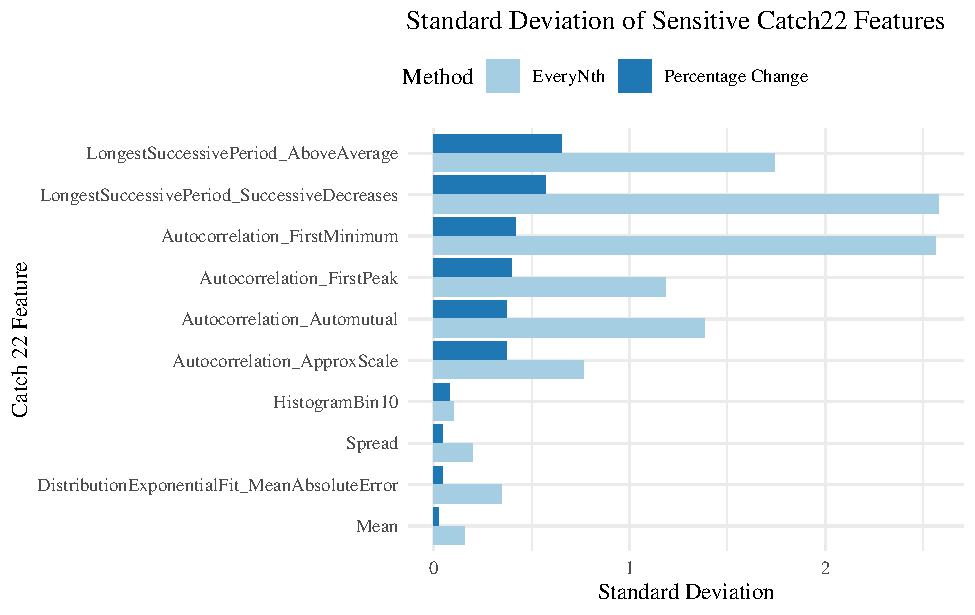
\includegraphics{210431461_CSC8639_Dissertation_files/figure-latex/CombinedSensitivity-1.pdf}

This visualisation highlights that approximately half of the catch22
time series features are noticeably impacted by both downsampling
algorithms. The \emph{EveryNth} algorithm impacts more features than
\emph{Percentage Change}; this is likely to be because more data is
discarded by the former algorithm than the latter in the 50 parameters
explored by this research. It would be beneficial to explore this
difference with further iterations of \emph{Percentage Change}
downsampling across the time series to understand its impact after more
data is discarded. For parameters 1 to 50, the different impacts of the
two downsampling algorithms on the ten most sensitive features for each
time series are presented in Annex B.

The values of catch22 features appear to increase as data is discarded.
It would be beneficial to explore this dynamic further; the analysis on
this dynamic conducted as part of this research is presented in Annex C.
The \emph{EveryNth} algorithm discards more data, more quickly, by
comparison to \emph{Percentage Change} algorithm. This creates acute
differences in the imputed time series which are discussed in the next
section.

\textbf{5.2 Feature Variation}

\emph{5.2a First Minimum of the Autocorrelation Function}

The catch22 feature with the highest standard deviation across the 900
time series is the first minimum of the autocorrelation function
(`Autocorr\_FirstMinimum' or `CO\_FirstMin\_ac'. This feature represents
``the number of steps into the future at which a value of the time
series at the current point and that future point remain substantially
(\textgreater1/e) correlated''
\protect\hyperlink{ref-feature_book}{\textbf{feature\_book?}}. The line
graphs below highlight how this feature changes over the time series
interpolated from different volumes of data after both downsampling
algorithms were applied. The difference between the catch22 feature
value of the original and imputed time series has been scaled for better
comparisons.

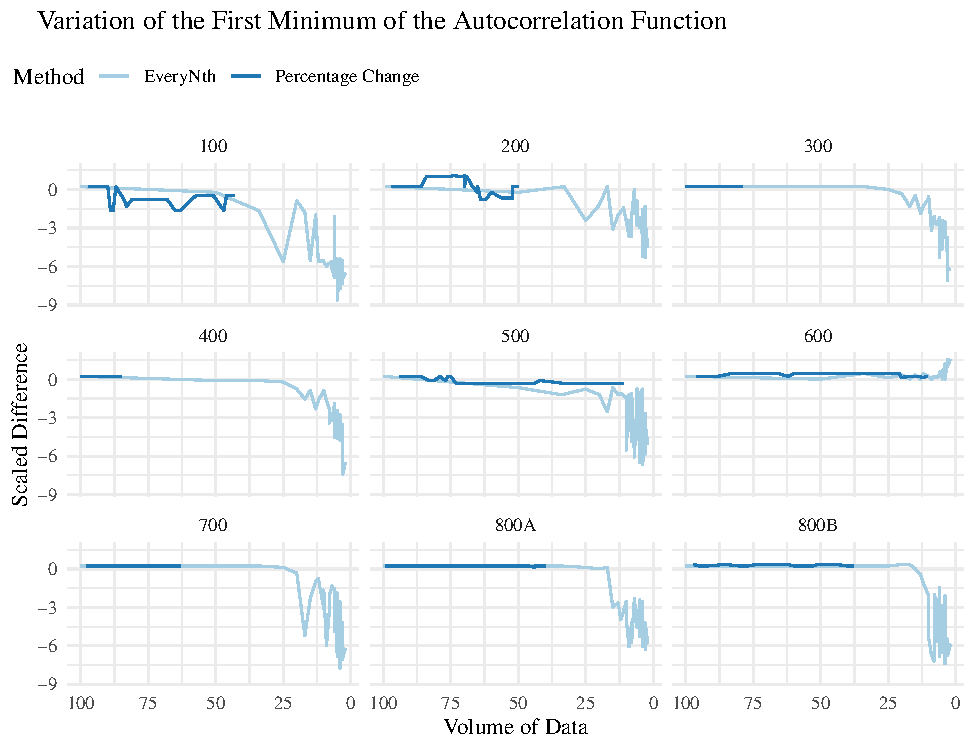
\includegraphics{210431461_CSC8639_Dissertation_files/figure-latex/FirstMinimum-1.pdf}

The visualisation clearly presents the impact of discarding data in
downsampling algorithms. The volume of data retained by \emph{Percentage
Change} algorithm varies by the type of time series whereas the volume
of data retained by the \emph{EveryNth} algorithm ends close to zero for
all the time series with significant difference observable when the
remaining data volume is below 25.

Line graphs of the original time series are provided in Annex D to
support comparison. The original time series `100' and `200' are
similarly shaped, with `100' trending upwards and `200' experiencing a
noticeable drop towards the end of the time series. In the line graphs
below, it is observable that `100' and `200' are similarly impacted by
\emph{EveryNth} and \emph{Percentage Change}, respectively. The impact
of \emph{Percentage Change} is more acute and variable than for the
other time series.

The original time series `300' and `400' are similarly shaped, with
significant peaks and troughs that start earlier for `400'. This is
likely to account for why \emph{Percentage Change} retains more data,
causing a negible impact on the catch22 feature for these time series.
The time series `500' and `600' are particularly distinct with some
obvious outliers in `500' and a gradual trend upwards for `600'. More
data is discarded by the \emph{Percentage Change} algorithm for these
time series than any of the others. Interestingly, `600' appears to be
the only time series for which the scaled difference between the
original and imputed catch22 feature values trends positively.

The remaining original time series `700', `800A' and `800B' are
distinct, but have similar slow-varying oscillation. This is mirrored by
the impacts of \emph{EveryNth} and \emph{Percentage Change}. The scaled
difference of the catch22 feature for the \emph{EveryNth} algorithm in
`700' has the widest spread of three and \emph{Percentage Change}
appears to retain more data than in `800A' and `800B'. Again, this is
likley to be because the changes in the peaks and troughs are more acute
in the original data.

\emph{5.2b Longest Sequence of Successive Steps that Decrease}

The feature with the second highest standard deviation across the 900
time series is the longest sequence of successive steps that decrease
(`LongestPeriod\_Decrease' or `SB\_BinaryStats\_diff\_longstretch0').
This catch22 feature ``calculates the longest sequence of successive
steps in the time series that decrease''
\protect\hyperlink{ref-feature_book}{\textbf{feature\_book?}}.

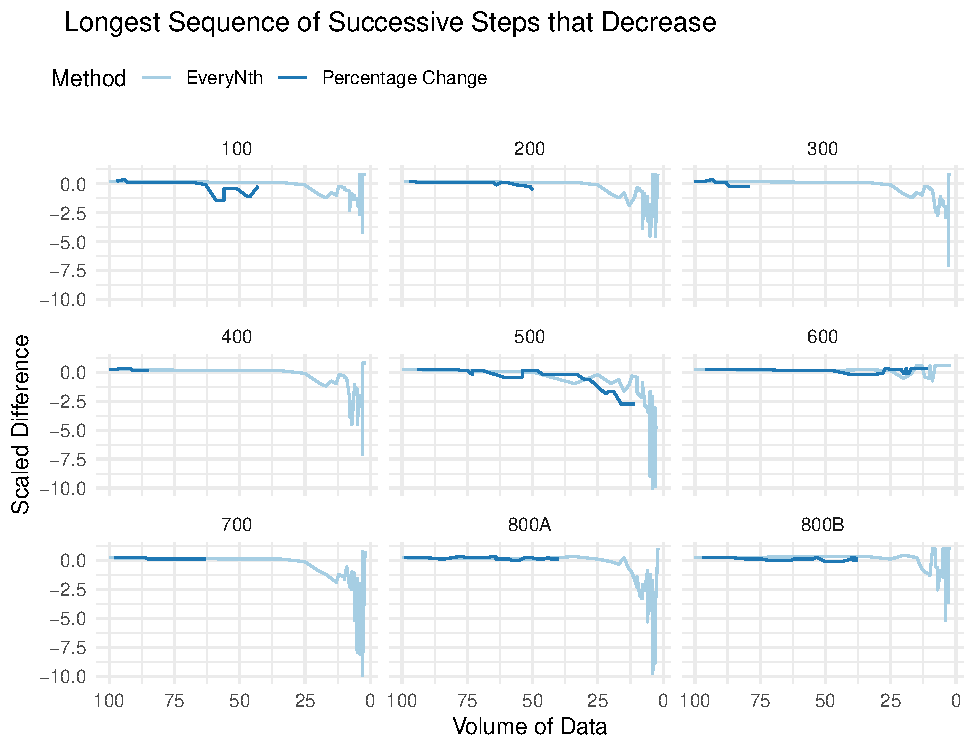
\includegraphics{210431461_CSC8639_Dissertation_files/figure-latex/LongestDecrease-1.pdf}

\emph{5.2c Longest Sequence of Successive Values Greater than the Mean}

The feature with the third highest standard deviation across the 900
time series is the longest sequence of successive values greater than
the mean (`LongestPeriod\_AboveAverage' or
`SB\_BinaryStats\_mean\_longstretch1'). This catch22 feature
``calculates the longest successive period of above average values''
\protect\hyperlink{ref-feature_book}{\textbf{feature\_book?}}.

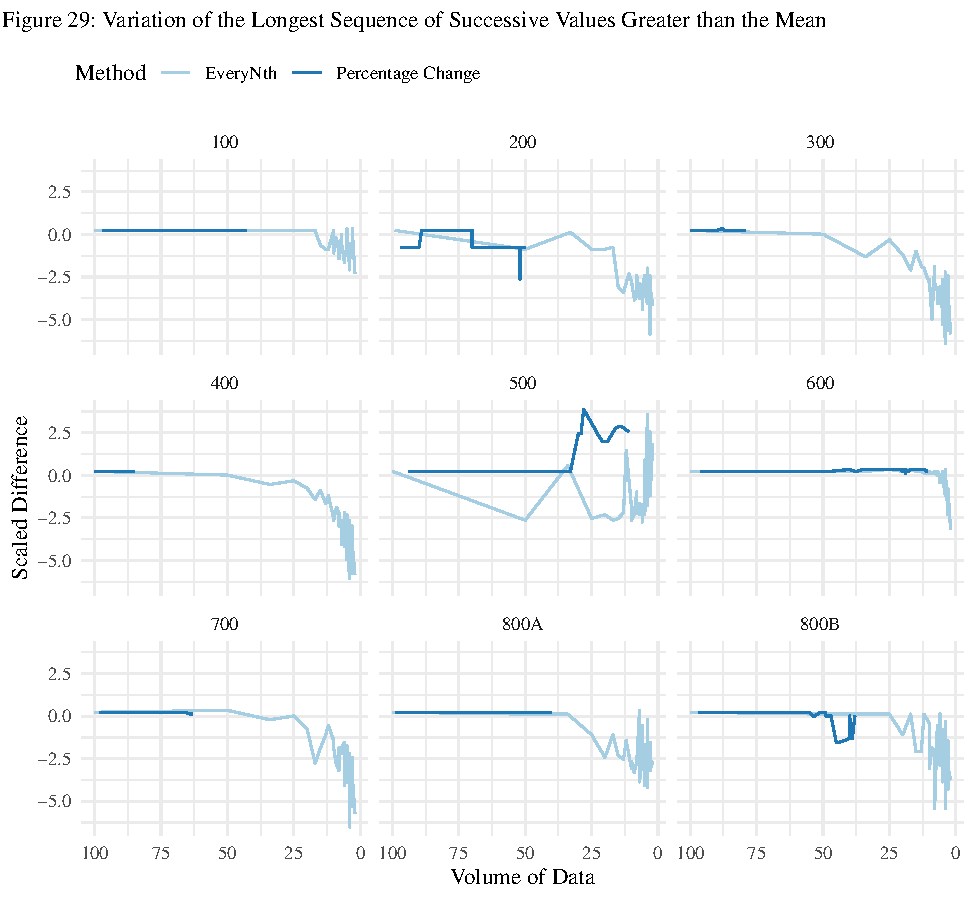
\includegraphics{210431461_CSC8639_Dissertation_files/figure-latex/LongestGreater-1.pdf}

\emph{5.2d Minimum of the Automutual Information Function}

The feature with the fourth highest standard deviation across the 900
time series is the minimum of the automutual information function
(`Autocorr\_Automutual' or
`IN\_AutoMutualInfoStats\_40\_gaussian\_fmmi'). This catch22 feature
outputs a measure of ``autocorrelation in the time series, as the
minimum of the automutual information function''
\protect\hyperlink{ref-feature_book}{\textbf{feature\_book?}}.

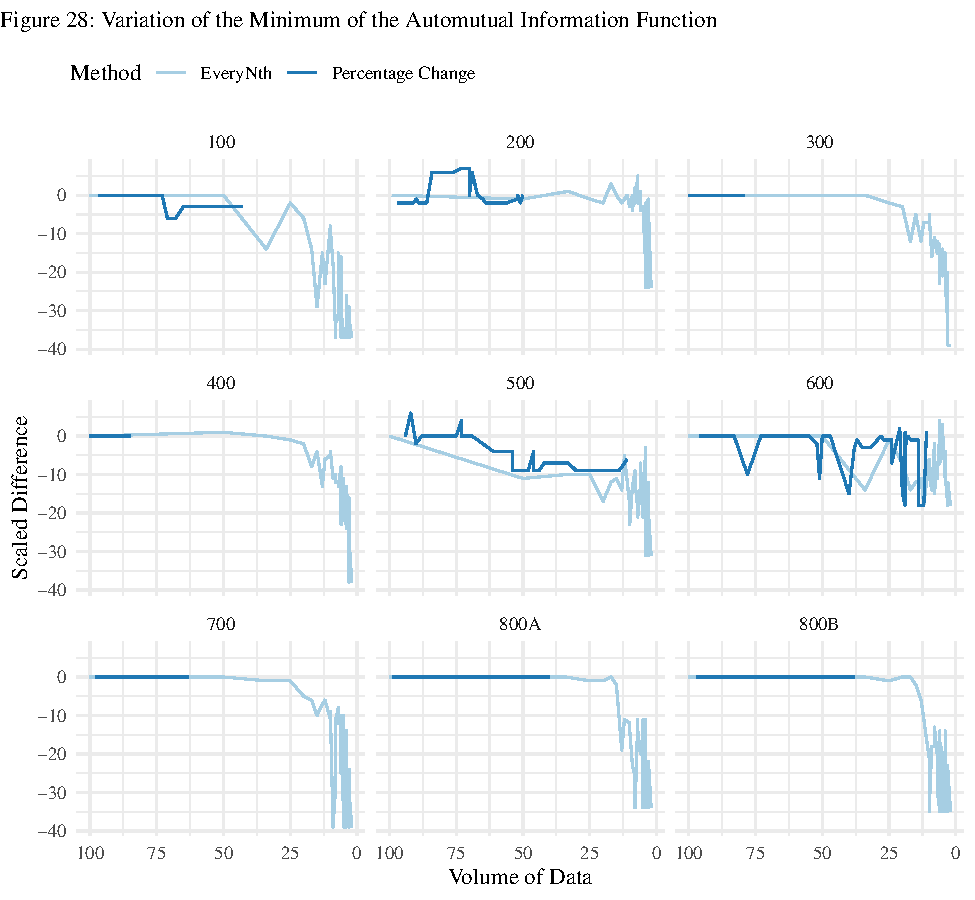
\includegraphics{210431461_CSC8639_Dissertation_files/figure-latex/AutoMutalFunction-1.pdf}

\emph{5.2e First Peak in the Autocorrelation Function}

The feature with the fifth highest standard deviation across the 900
time series is the first peak in the autocorrelation function
(`Autocorr\_FirstPeak' or `PD\_PeriodicityWang\_th0\_01'). This catch22
feature ``returns the first peak in the autocorrelation function
satisfying a set of conditions (after detrending the time series using a
single-knot cubic regression spline)''
\protect\hyperlink{ref-feature_book}{\textbf{feature\_book?}}. In
general, the feature returns higher values for slower time series
oscillation.

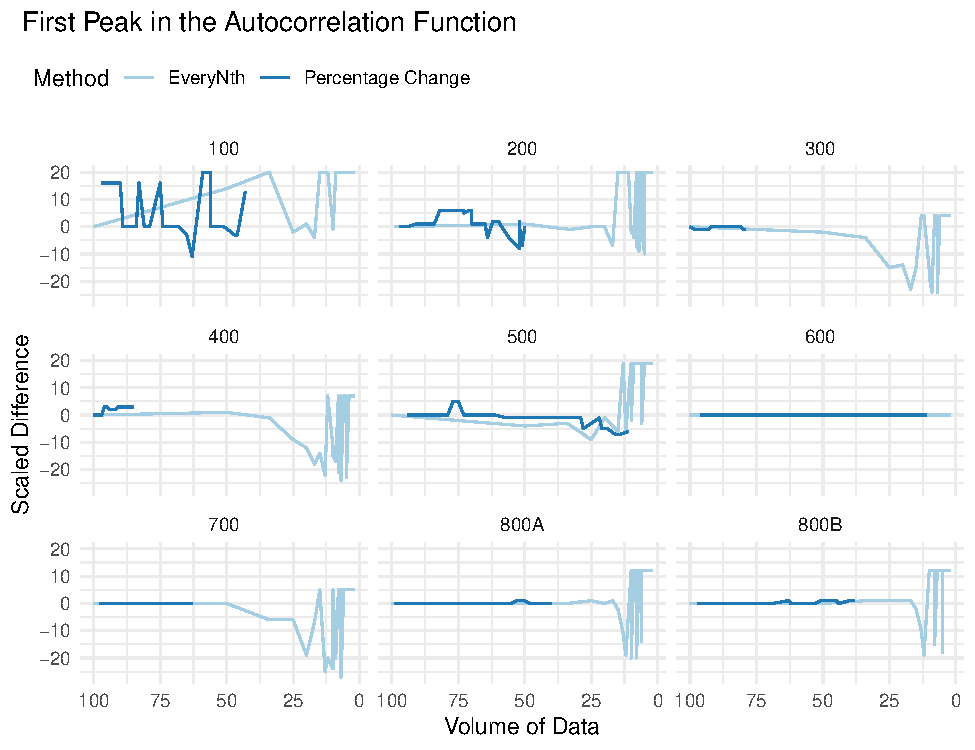
\includegraphics{210431461_CSC8639_Dissertation_files/figure-latex/FirstPeak-1.pdf}

\emph{5.2f Approximate Scale of Autocorrelation}

The feature with the sixth highest standard deviation across the 900
time series is the approximate scale of autocorrelation
(`Autocorr\_ApproxScale' or `CO\_f1ecac'). This catch22 feature
``computes the first 1/e crossing of the autocorrelation function of the
time series''
\protect\hyperlink{ref-feature_book}{\textbf{feature\_book?}}. It is
similar to the first minimum of the autocorrelation function.

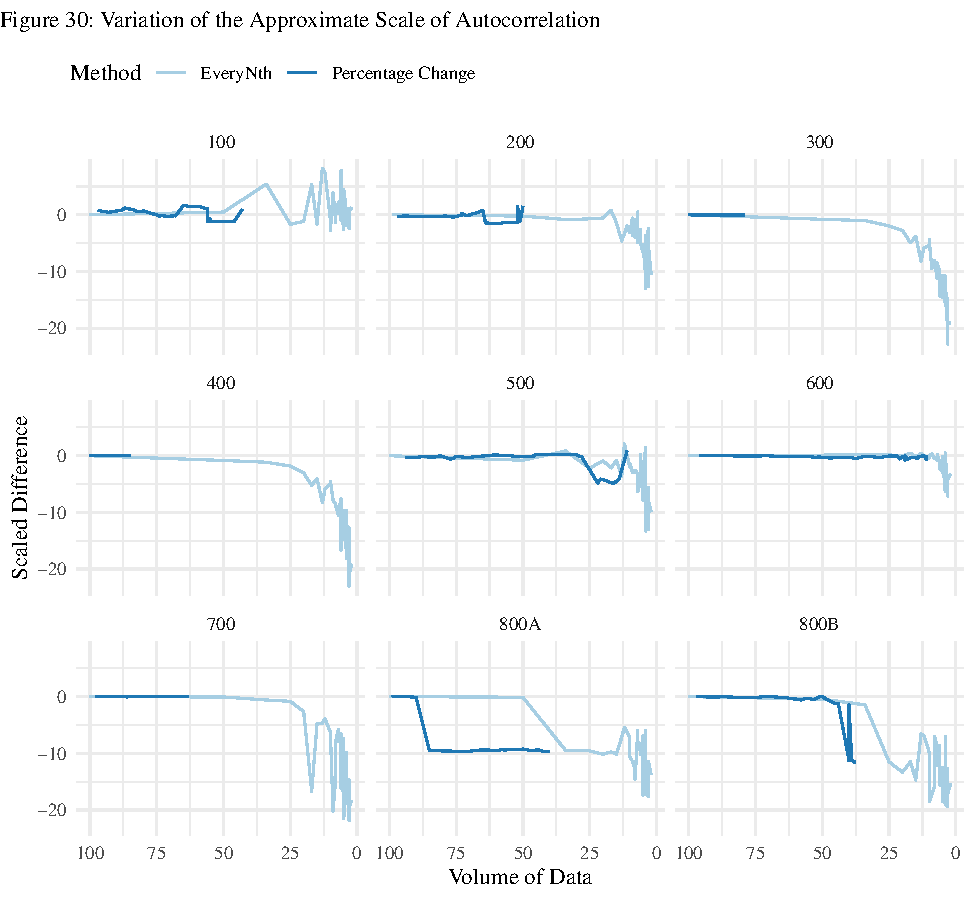
\includegraphics{210431461_CSC8639_Dissertation_files/figure-latex/ApproxScale-1.pdf}

\emph{5.2g Mean Absolute Error of an Exponential Fit}

The feature with the seventh highest standard deviation across the 900
time series is the approximate scale of autocorrelation
(`DistributionExponentialFit\_MAE' or
`CO\_Embed2\_Dist\_tau\_d\_expfit\_meandiff'). This catch22 feature
outputs the mean absolute error of an exponential fit to a distribution
which is calculated by representing ``the time series in a
two-dimensional time-delay embedding space (using a time delay equal to
the first zero-crossing of the autocorrelation function)\ldots{} {[}then
computing the{]} successive distances between points in this 2D
embedding space and analyzes the probability distribution of these
distances''
\protect\hyperlink{ref-feature_book}{\textbf{feature\_book?}}.

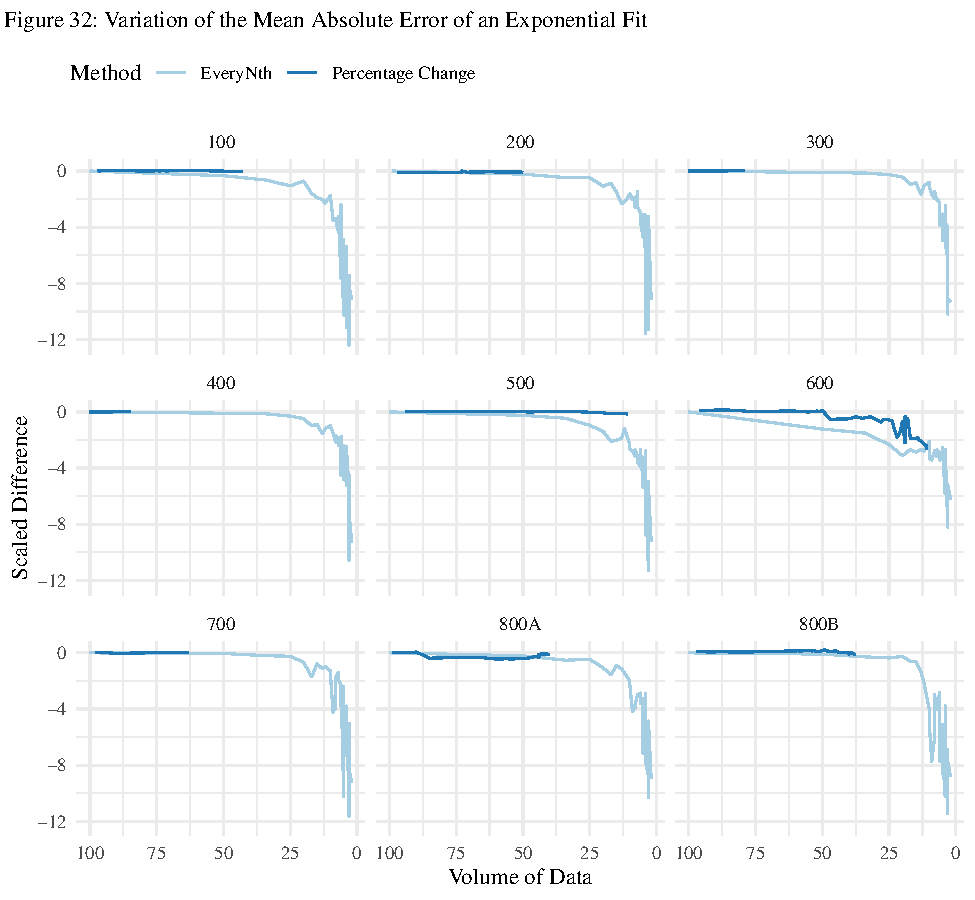
\includegraphics{210431461_CSC8639_Dissertation_files/figure-latex/MAE-1.pdf}

\hypertarget{future-work}{%
\section{FUTURE WORK}\label{future-work}}

\label{sec:headings}

The data pipeline developed by C. H. Lubba et. al could be used to
generate other subsets of time series features for distinct tasks in any
domain. This is likely to be important for highly specialised tasks or
domains.

Highlight in text: - The values of catch22 features appear to increase
as data is discarded. It would be beneficial to explore this dynamic
further; - he \emph{EveryNth} algorithm impacts more features than
\emph{Percentage Change}; this is likely to be because more data is
discarded by the former algorithm than the latter in the 50 parameters
explored by this research. It would be beneficial to explore this
difference with further iterations of \emph{Percentage Change}
downsampling across the time series to understand its impact after more
data is discarded.

\hypertarget{conclusion}{%
\section{CONCLUSION}\label{conclusion}}

\label{sec:headings}

\hypertarget{references}{%
\section{REFERENCES}\label{references}}

\label{sec:headings}

\hypertarget{annex-a-sensitivity-of-catch22-features}{%
\section{Annex A: Sensitivity of Catch22
Features}\label{annex-a-sensitivity-of-catch22-features}}

\begin{Shaded}
\begin{Highlighting}[]
\CommentTok{\# Reshape sensitivity subset data to a long format}
\NormalTok{subset\_sensitivity\_joined\_long }\OtherTok{\textless{}{-}}\NormalTok{ subset\_sensitivity\_joined }\SpecialCharTok{\%\textgreater{}\%}
  \FunctionTok{pivot\_longer}\NormalTok{(}\AttributeTok{cols =} \FunctionTok{c}\NormalTok{(everyNthSensitivity, PercentageChangeSensitivity), }
               \AttributeTok{names\_to =} \StringTok{"Method"}\NormalTok{, }
               \AttributeTok{values\_to =} \StringTok{"StandardDeviation"}\NormalTok{)}

\CommentTok{\# Change the Method into a factor and set the levels}
\NormalTok{subset\_sensitivity\_joined\_long}\SpecialCharTok{$}\NormalTok{Method }\OtherTok{\textless{}{-}} \FunctionTok{factor}\NormalTok{(subset\_sensitivity\_joined\_long}\SpecialCharTok{$}\NormalTok{Method, }\AttributeTok{levels =} \FunctionTok{c}\NormalTok{(}\StringTok{"PercentageChangeSensitivity"}\NormalTok{, }\StringTok{"everyNthSensitivity"}\NormalTok{))}

\CommentTok{\# Recode the names of the Methods}
\NormalTok{subset\_sensitivity\_joined\_long}\SpecialCharTok{$}\NormalTok{Method }\OtherTok{\textless{}{-}} \FunctionTok{recode}\NormalTok{(subset\_sensitivity\_joined\_long}\SpecialCharTok{$}\NormalTok{Method,  }
                                                \StringTok{"PercentageChangeSensitivity"} \OtherTok{=} \StringTok{"Percentage Change"}\NormalTok{, }
                                                \StringTok{"everyNthSensitivity"} \OtherTok{=} \StringTok{"EveryNth"}\NormalTok{)}
\CommentTok{\# Recode the names of the Rcatch22 features}
\NormalTok{subset\_sensitivity\_joined\_long}\SpecialCharTok{$}\NormalTok{names }\OtherTok{\textless{}{-}} \FunctionTok{recode}\NormalTok{(subset\_sensitivity\_joined\_long}\SpecialCharTok{$}\NormalTok{names,  }
                                               \StringTok{\textquotesingle{}CO\_f1ecac\textquotesingle{}} \OtherTok{=} \StringTok{"Autocorrelation\_ApproxScale"}\NormalTok{,}
                                               \StringTok{\textquotesingle{}CO\_FirstMin\_ac\textquotesingle{}} \OtherTok{=} \StringTok{"Autocorrelation\_FirstMinimum"}\NormalTok{,}
                                               \StringTok{\textquotesingle{}SB\_BinaryStats\_mean\_longstretch1\textquotesingle{}} \OtherTok{=} \StringTok{"LongestSuccessivePeriod\_AboveAverage"}\NormalTok{,}
                                               \StringTok{\textquotesingle{}PD\_PeriodicityWang\_th0\_01\textquotesingle{}} \OtherTok{=} \StringTok{"Autocorrelation\_FirstPeak"}\NormalTok{,}
                                               \StringTok{\textquotesingle{}DN\_Mean\textquotesingle{}} \OtherTok{=} \StringTok{\textquotesingle{}Mean\textquotesingle{}}\NormalTok{,}
                                               \StringTok{\textquotesingle{}DN\_HistogramMode\_10\textquotesingle{}} \OtherTok{=} \StringTok{"HistogramBin10"}\NormalTok{,}
                                               \StringTok{\textquotesingle{}DN\_Spread\_Std\textquotesingle{}} \OtherTok{=} \StringTok{\textquotesingle{}Spead\textquotesingle{}}\NormalTok{,}
                                               \StringTok{\textquotesingle{}CO\_Embed2\_Dist\_tau\_d\_expfit\_meandiff\textquotesingle{}} \OtherTok{=} \StringTok{"DistributionExponentialFit\_MeanAbsoluteError"}\NormalTok{,}
                                               \StringTok{\textquotesingle{}IN\_AutoMutualInfoStats\_40\_gaussian\_fmmi\textquotesingle{}} \OtherTok{=} \StringTok{"Autocorrelation\_Automutual"}\NormalTok{,}
                                               \StringTok{\textquotesingle{}SB\_BinaryStats\_diff\_longstretch0\textquotesingle{}} \OtherTok{=} \StringTok{"LongestSuccessivePeriod\_SuccessiveDecreases"}\NormalTok{)}

\CommentTok{\# Create a bar plot}
\NormalTok{sensitive\_subset\_plot }\OtherTok{\textless{}{-}} \FunctionTok{ggplot}\NormalTok{(subset\_sensitivity\_joined\_long, }\FunctionTok{aes}\NormalTok{(}\AttributeTok{x =}\NormalTok{ StandardDeviation, }\AttributeTok{y =}\NormalTok{ names, }\AttributeTok{fill =}\NormalTok{ Method)) }\SpecialCharTok{+}
  \FunctionTok{geom\_bar}\NormalTok{(}\AttributeTok{stat =} \StringTok{"identity"}\NormalTok{, }\AttributeTok{position =} \FunctionTok{position\_dodge}\NormalTok{()) }\SpecialCharTok{+}
  \FunctionTok{theme\_minimal}\NormalTok{() }\SpecialCharTok{+}
  \FunctionTok{theme}\NormalTok{(}\AttributeTok{text =} \FunctionTok{element\_text}\NormalTok{(}\AttributeTok{size =} \DecValTok{30}\NormalTok{), }\AttributeTok{legend.position =} \StringTok{"top"}\NormalTok{) }\SpecialCharTok{+}
  \FunctionTok{labs}\NormalTok{(}\AttributeTok{x =} \StringTok{"Standard Deviation"}\NormalTok{, }\AttributeTok{y =} \StringTok{"Catch22 Feature"}\NormalTok{, }\AttributeTok{fill =} \StringTok{"Method"}\NormalTok{, }\AttributeTok{title =} \StringTok{"Standard Deviation of Most Sensitive Features"}\NormalTok{) }\SpecialCharTok{+}
  \FunctionTok{scale\_fill\_brewer}\NormalTok{(}\AttributeTok{palette =} \StringTok{"Paired"}\NormalTok{) }\SpecialCharTok{+}
  \FunctionTok{scale\_x\_continuous}\NormalTok{(}\AttributeTok{limits =} \FunctionTok{c}\NormalTok{(}\DecValTok{0}\NormalTok{, }\ConstantTok{NA}\NormalTok{))}
\end{Highlighting}
\end{Shaded}

\begin{Shaded}
\begin{Highlighting}[]
\NormalTok{knitr}\SpecialCharTok{::}\FunctionTok{kable}\NormalTok{((sensitivity\_joined), }\AttributeTok{caption =} \StringTok{"Sensitivity of Catch22 Features to EveryNth and Percentage Change Downsampling"}\NormalTok{)}
\end{Highlighting}
\end{Shaded}

\begin{longtable}[]{@{}
  >{\raggedright\arraybackslash}p{(\columnwidth - 4\tabcolsep) * \real{0.4783}}
  >{\raggedleft\arraybackslash}p{(\columnwidth - 4\tabcolsep) * \real{0.2174}}
  >{\raggedleft\arraybackslash}p{(\columnwidth - 4\tabcolsep) * \real{0.3043}}@{}}
\caption{Sensitivity of Catch22 Features to EveryNth and Percentage
Change Downsampling}\tabularnewline
\toprule\noalign{}
\begin{minipage}[b]{\linewidth}\raggedright
names
\end{minipage} & \begin{minipage}[b]{\linewidth}\raggedleft
everyNthSensitivity
\end{minipage} & \begin{minipage}[b]{\linewidth}\raggedleft
PercentageChangeSensitivity
\end{minipage} \\
\midrule\noalign{}
\endfirsthead
\toprule\noalign{}
\begin{minipage}[b]{\linewidth}\raggedright
names
\end{minipage} & \begin{minipage}[b]{\linewidth}\raggedleft
everyNthSensitivity
\end{minipage} & \begin{minipage}[b]{\linewidth}\raggedleft
PercentageChangeSensitivity
\end{minipage} \\
\midrule\noalign{}
\endhead
\bottomrule\noalign{}
\endlastfoot
SB\_BinaryStats\_diff\_longstretch0 & 2.5778227 & 0.5711553 \\
CO\_FirstMin\_ac & 2.5639294 & 0.4181318 \\
SB\_BinaryStats\_mean\_longstretch1 & 1.7389139 & 0.6524714 \\
IN\_AutoMutualInfoStats\_40\_gaussian\_fmmi & 1.3808674 & 0.3736266 \\
PD\_PeriodicityWang\_th0\_01 & 1.1844657 & 0.3954080 \\
CO\_f1ecac & 0.7661026 & 0.3713025 \\
CO\_Embed2\_Dist\_tau\_d\_expfit\_meandiff & 0.3440829 & 0.0437543 \\
DN\_Spread\_Std & 0.1985249 & 0.0455823 \\
DN\_Mean & 0.1572628 & 0.0227554 \\
DN\_HistogramMode\_10 & 0.1013119 & 0.0822124 \\
DN\_HistogramMode\_5 & 0.0869504 & 0.0647597 \\
SP\_Summaries\_welch\_rect\_centroid & 0.0654187 & 0.0025698 \\
FC\_LocalSimple\_mean1\_tauresrat & 0.0436216 & 0.0218936 \\
DN\_OutlierInclude\_n\_001\_mdrmd & 0.0434259 & 0.0050690 \\
SC\_FluctAnal\_2\_rsrangefit\_50\_1\_logi\_prop\_r1 & 0.0432552 &
0.0277534 \\
CO\_trev\_1\_num & 0.0425513 & 0.0130514 \\
FC\_LocalSimple\_mean3\_stderr & 0.0384460 & 0.0049473 \\
DN\_OutlierInclude\_p\_001\_mdrmd & 0.0349796 & 0.0138568 \\
SB\_MotifThree\_quantile\_hh & 0.0340103 & 0.0139764 \\
SP\_Summaries\_welch\_rect\_area\_5\_1 & 0.0326959 & 0.0038222 \\
CO\_HistogramAMI\_even\_2\_5 & 0.0315734 & 0.0134047 \\
MD\_hrv\_classic\_pnn40 & 0.0241202 & 0.0102366 \\
SC\_FluctAnal\_2\_dfa\_50\_1\_2\_logi\_prop\_r1 & 0.0224893 &
0.0087991 \\
SB\_TransitionMatrix\_3ac\_sumdiagcov & 0.0053928 & 0.0037061 \\
\end{longtable}

\hypertarget{annex-b-top-ten-most-sensitive-catch22-features}{%
\section{Annex B: Top Ten Most Sensitive Catch22
Features}\label{annex-b-top-ten-most-sensitive-catch22-features}}

The ten features most impacted by both downsampling algorithms are
selected for further investigation. The bar graph below visualises the
standard deviation of the \emph{EveryNth} algorithm for these features
across all the parameters for each of the nine synthetic time series.

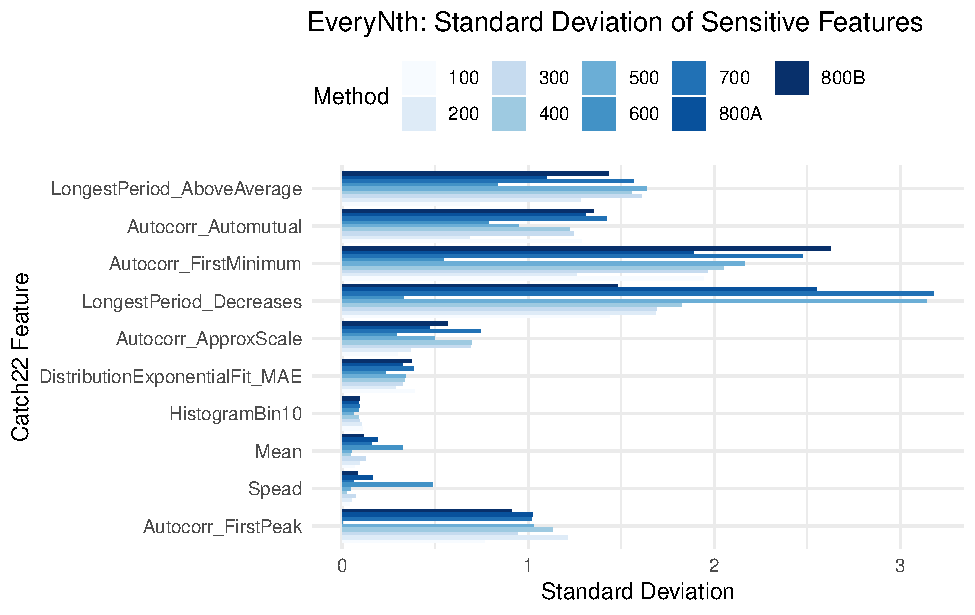
\includegraphics{210431461_CSC8639_Dissertation_files/figure-latex/NthSensitivity-1.pdf}

The visualisation above highlights that the impact of downsampling on
each catch22 feature is different for each time series type. This holds
true for the \emph{Percentage Change} algorithm too. The bar graph below
visualises the standard deviation for the same ten features across all
the parameters for each of the nine synthetic time series.

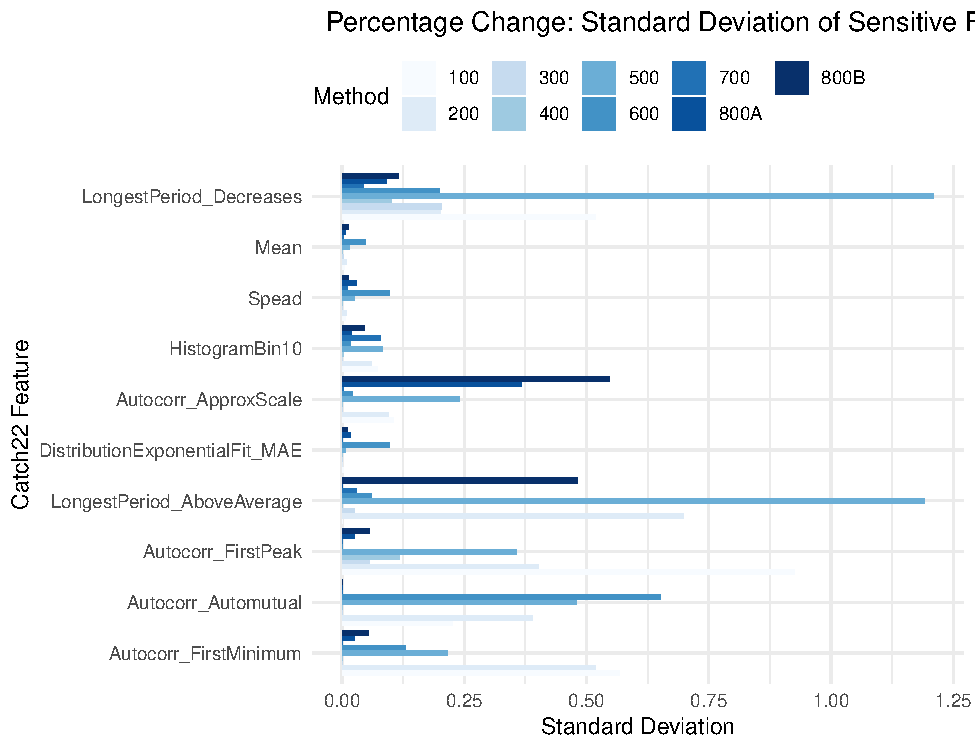
\includegraphics{210431461_CSC8639_Dissertation_files/figure-latex/PCSensitivity-1.pdf}

Interestingly, the impact of \emph{Percentage Change} on many of these
features is acute despite the spread of standard deviation being
smaller. For example\ldots{} {[}ADD OBSERVATION{]}

\hypertarget{annex-c-data-volume-vs.-downsampling-parameters}{%
\section{Annex C: Data Volume vs.~Downsampling
Parameters}\label{annex-c-data-volume-vs.-downsampling-parameters}}

To better compare this impact, the heatmap below visualises the scaled
difference between the original and imputed time series by the data
volume remaining after each downsampling algorithm is applied. Annex B
shares this graph with downsampling parameter instead of data volume to
explain why data volume was chosen.

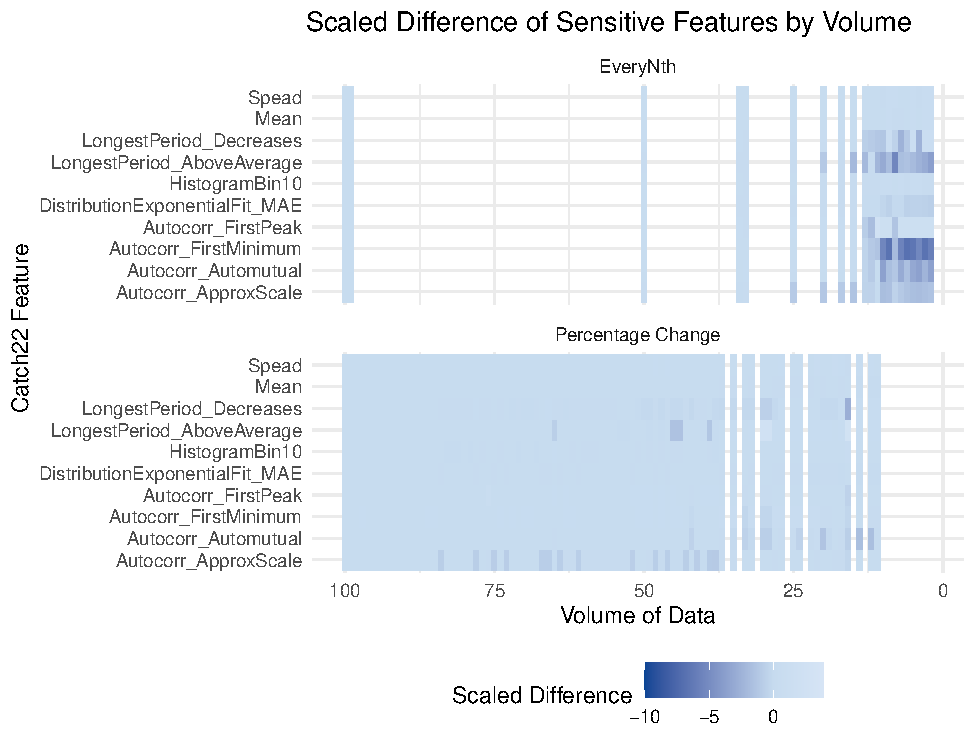
\includegraphics{210431461_CSC8639_Dissertation_files/figure-latex/Heatmap-1.pdf}

Interestingly, this visualisation demonstrated that the catch22 features
that are impacted by both downsampling algorithms tend to increase in
comparison the original feature values. The visualisation emphasises how
quickly \emph{EveryNth} discards data by comparison to \emph{Percentage
Change}. This creates acute differences in the imputed time series
created when less than 20 data points remained after \emph{EveryNth} is
applied. For both downsampling algorithms, the `Autocorr\_ApproxScale'
and `LongestPeriod\_AboveAverage' appear to be the first features to be
impacted. {[}EXPLAIN FEATURES{]}. The impact on both features appears to
be inconsistent when \emph{Percentage Change} is applied before linear
interpolation. For example, the are data volumes where
\texttt{Autocorr\_ApproxScale} and \texttt{LongestPeriod\_AboveAverage}
do not appear to be impacted by \emph{Percentage Change} when higher
date volumes appear to be impacted.

\hypertarget{refs}{}
\begin{CSLReferences}{0}{0}
\leavevmode\vadjust pre{\hypertarget{ref-data2017}{}}%
\CSLLeftMargin{{[}1{]} }%
\CSLRightInline{Cabinet Office and Government Digital Service,
{``Government transformation strategy: Better use of data.''} HM
Government;
\url{https://www.gov.uk/government/publications/government-transformation-strategy-2017-to-2020/government-transformation-strategy-better-use-of-data},
2017.}

\leavevmode\vadjust pre{\hypertarget{ref-data2020}{}}%
\CSLLeftMargin{{[}2{]} }%
\CSLRightInline{Department for Digital, Culture, Media \& Sport and
Department for Science, Innovation \& Technology, {``National data
strategy.''} HM Government;
\url{https://www.gov.uk/government/publications/uk-national-data-strategy/national-data-strategy},
2020.}

\leavevmode\vadjust pre{\hypertarget{ref-data2021}{}}%
\CSLLeftMargin{{[}3{]} }%
\CSLRightInline{M. of Defence, {``Data strategy for defence,''}
\emph{GOV.UK}. HM Government;
\url{https://www.gov.uk/government/publications/data-strategy-for-defence/data-strategy-for-defence},
2021.}

\leavevmode\vadjust pre{\hypertarget{ref-data2022}{}}%
\CSLLeftMargin{{[}4{]} }%
\CSLRightInline{Central Digital \& Data Office, {``Transforming for a
digital future: 2022 to 2025 roadmap for digital and data.''} HM
Government;
\url{https://www.gov.uk/government/publications/roadmap-for-digital-and-data-2022-to-2025/transforming-for-a-digital-future-2022-to-2025-roadmap-for-digital-and-data},
2022.}

\leavevmode\vadjust pre{\hypertarget{ref-trust}{}}%
\CSLLeftMargin{{[}5{]} }%
\CSLRightInline{Centre for Data Ethics \& Innovation, {``Addressing
trust in public sector data use.''}
\url{https://www.gov.uk/government/publications/cdei-publishes-its-first-report-on-public-sector-data-sharing/addressing-trust-in-public-sector-data-use\#introduction--context}.}

\leavevmode\vadjust pre{\hypertarget{ref-pathway}{}}%
\CSLLeftMargin{{[}6{]} }%
\CSLRightInline{Government Analysis Function, {``Types of data in
government learning pathway.''}
\url{https://analysisfunction.civilservice.gov.uk/learning-development/learning-pathways/types-of-data-in-government-learning-pathway/},
2022.}

\leavevmode\vadjust pre{\hypertarget{ref-onstool}{}}%
\CSLLeftMargin{{[}7{]} }%
\CSLRightInline{Office for National Statistics, {``Time series
explorer.''}
\url{https://www.ons.gov.uk/timeseriestool?query=\&topic=\&updated=\&fromDateDay=\&fromDateMonth=\&fromDateYear=\&toDateDay=\&toDateMonth=\&toDateYear=\&size=50},
Unknown.}

\leavevmode\vadjust pre{\hypertarget{ref-TVStore}{}}%
\CSLLeftMargin{{[}8{]} }%
\CSLRightInline{Y. An, Y. Su, Y. Zhu, and J. Wang, {``TVStore:
Automatically bounding time series storage via time-varying
compression,''} in \emph{Proceedings of the 20th USENIX conference on
file and storage technologies}, in USENIX conference on file and STorage
technologies. Santa Clara, CA, USA: USENIX Association, 2022, pp.
83--99.}

\leavevmode\vadjust pre{\hypertarget{ref-datapoint}{}}%
\CSLLeftMargin{{[}9{]} }%
\CSLRightInline{J. Donckt, J. Donckt, M. Rademaker, and S. Hoecke,
{``Data point selection for line chart visualization: Methodological
assessment and evidence-based guidelines.''} 2023. doi:
\href{https://doi.org/10.48550/arXiv.2304.00900}{10.48550/arXiv.2304.00900}.}

\leavevmode\vadjust pre{\hypertarget{ref-Sveinn}{}}%
\CSLLeftMargin{{[}10{]} }%
\CSLRightInline{S. Steinarsson, {``Downsampling time series for visual
representation.''} University of Iceland, Faculty of Industrial
Engineering, Mechanical Engineering; Computer Science, School of
Engineering; Natural Sciences, University of Iceland, Reykjavik,
Iceland, 2013.}

\leavevmode\vadjust pre{\hypertarget{ref-Shift}{}}%
\CSLLeftMargin{{[}11{]} }%
\CSLRightInline{The Shift Project, {``Implementing digital
sufficiency,''} 2020.}

\leavevmode\vadjust pre{\hypertarget{ref-downsampling}{}}%
\CSLLeftMargin{{[}12{]} }%
\CSLRightInline{W. Aigner, S. Miksch, W. Muller, H. Schumann, and C.
Tominski, {``Visual methods for analyzing time-oriented data,''}
\emph{IEEE Transactions on Visualization and Computer Graphics}, vol.
14, no. 1, pp. 47--60, 2008, doi:
\href{https://doi.org/10.1109/TVCG.2007.70415}{10.1109/TVCG.2007.70415}.}

\leavevmode\vadjust pre{\hypertarget{ref-sampling}{}}%
\CSLLeftMargin{{[}13{]} }%
\CSLRightInline{B. C. Kwon, J. Verma, P. J. Haas, and C. Demiralp,
{``Sampling for scalable visual analytics,''} \emph{IEEE Computer
Graphics and Applications}, vol. 37, no. 1, pp. 100--108, 2017, doi:
\href{https://doi.org/10.1109/MCG.2017.6}{10.1109/MCG.2017.6}.}

\leavevmode\vadjust pre{\hypertarget{ref-MinMaxLTTB}{}}%
\CSLLeftMargin{{[}14{]} }%
\CSLRightInline{J. Donckt, J. Donckt, M. Rademaker, and S. Hoecke,
{``MinMaxLTTB: Leveraging MinMax-preselection to scale LTTB.''} 2023.
Available: \url{https://arxiv.org/abs/2305.00332}}

\leavevmode\vadjust pre{\hypertarget{ref-imputeTS_R}{}}%
\CSLLeftMargin{{[}15{]} }%
\CSLRightInline{S. Moritz and T. Bartiz-Beielstein, {``imputeTS: Time
series missing value imputation in r,''} vol. 9.1. R Journal, 2017. doi:
\href{https://doi.org/10.32614/RJ-2017-009}{10.32614/RJ-2017-009}.}

\leavevmode\vadjust pre{\hypertarget{ref-catch22_R}{}}%
\CSLLeftMargin{{[}16{]} }%
\CSLRightInline{C. H. Lubba, B. Fulcher, T. Henderspn, B. Harris, O. r.
TL, and O. Cliff, {``catch22: CAnonical time-series CHaracteristics.''}
R Journal, 2022. doi:
\href{https://doi.org/10.5281/zenodo.6673597}{10.5281/zenodo.6673597}.}

\leavevmode\vadjust pre{\hypertarget{ref-political_transparency}{}}%
\CSLLeftMargin{{[}17{]} }%
\CSLRightInline{K. E. Levy and D. M. Johns, {``When open data is a
trojan horse: The weaponization of transparency in science and
governance,''} \emph{Big Data \& Society}, vol. 3, no. 1, 2016, doi:
\href{https://doi.org/10.1177/2053951715621568}{10.1177/2053951715621568}.}

\leavevmode\vadjust pre{\hypertarget{ref-social_transparency}{}}%
\CSLLeftMargin{{[}18{]} }%
\CSLRightInline{J. Bates, H. Kennedy, I. Medina Perea, S. Oman, and L.
Pinney, {``Socially meaningful transparency in data-based systems:
Reflections and proposals from practice,''} \emph{Journal of
Documentation}, vol. ahead--of--print, 2023, doi:
\href{https://doi.org/10.1108/JD-01-2023-0006}{10.1108/JD-01-2023-0006}.}

\leavevmode\vadjust pre{\hypertarget{ref-transparency_lack}{}}%
\CSLLeftMargin{{[}19{]} }%
\CSLRightInline{M. Ananny and K. Crawford, {``Seeing without knowing:
Limitations of the transparency ideal and its application to algorithmic
accountability,''} \emph{New Media \& Society}, vol. 20, no. 3, pp.
973--989, 2018, doi:
\href{https://doi.org/10.1177/1461444816676645}{10.1177/1461444816676645}.}

\leavevmode\vadjust pre{\hypertarget{ref-digital_transparency}{}}%
\CSLLeftMargin{{[}20{]} }%
\CSLRightInline{R. Matheus, M. Janssen, and T. Janowski, {``Design
principles for creating digital transparency in government,''}
\emph{Government Information Quarterly}, vol. 38, no. 1, 2021, doi:
\url{https://doi.org/10.1016/j.giq.2020.101550}.}

\leavevmode\vadjust pre{\hypertarget{ref-transparency_obfuscation}{}}%
\CSLLeftMargin{{[}21{]} }%
\CSLRightInline{N. A. Draper and J. Turow, {``The corporate cultivation
of digital resignation,''} \emph{New Media \& Society}, vol. 21, no. 8,
pp. 1824--1839, 2019, doi:
\href{https://doi.org/10.1177/1461444819833331}{10.1177/1461444819833331}.}

\leavevmode\vadjust pre{\hypertarget{ref-transparency_fallacy}{}}%
\CSLLeftMargin{{[}22{]} }%
\CSLRightInline{J. A. Obar, {``Sunlight alone is not a disinfectant:
Consent and the futility of opening big data black boxes (without
assistance),''} \emph{Big Data \& Society}, vol. 7, no. 1, 2020, doi:
\href{https://doi.org/10.1177/2053951720935615}{10.1177/2053951720935615}.}

\leavevmode\vadjust pre{\hypertarget{ref-timenotes}{}}%
\CSLLeftMargin{{[}23{]} }%
\CSLRightInline{J. Walker, R. Borgo, and MW. Jones, {``TimeNotes: A
study on effective chart visualization and interaction techniques for
time-series data,''} \emph{IEEE Transactions on Visualization and
Computer Graphics}, vol. 22, 2016, doi:
\href{https://doi.org/10.1109/TVCG.2015.2467751}{10.1109/TVCG.2015.2467751}.}

\leavevmode\vadjust pre{\hypertarget{ref-plotly}{}}%
\CSLLeftMargin{{[}24{]} }%
\CSLRightInline{J. Donckt, J. Donckt, E. Deprost, and S. Hoecke,
{``Plotly-resampler: Effective visual analytics for large time
series,''} \emph{IEEE Visualization and Visual Analytics}, 2022, doi:
\href{https://doi.org/10.1109/VIS54862.2022.00013}{10.1109/VIS54862.2022.00013}.}

\leavevmode\vadjust pre{\hypertarget{ref-imputeTS}{}}%
\CSLLeftMargin{{[}25{]} }%
\CSLRightInline{S. Moritz and T. Bartiz-Beielstein, {``imputeTS: Time
series missing value imputation in r.''} R Journal, 2017. Available:
\url{https://cran.r-project.org/web/packages/imputeTS/vignettes/imputeTS-Time-Series-Missing-Value-Imputation-in-R.pdf}}

\leavevmode\vadjust pre{\hypertarget{ref-storage}{}}%
\CSLLeftMargin{{[}26{]} }%
\CSLRightInline{A. Visheratin \emph{et al.}, {``Peregreen {\textendash}
modular database for efficient storage of historical time series in
cloud environments,''} in \emph{2020 USENIX annual technical conference
(USENIX ATC 20)}, USENIX Association, 2020, pp. 589--601. Available:
\url{https://www.usenix.org/conference/atc20/presentation/visheratin}}

\leavevmode\vadjust pre{\hypertarget{ref-CatchUp}{}}%
\CSLLeftMargin{{[}27{]} }%
\CSLRightInline{T. Schlossnagle, J. Sheehy, and C. McCubbin,
{``Always-on time-series database: Keeping up where there's no way to
catch up,''} \emph{Commun. ACM}, vol. 64, no. 7, pp. 50--56, 2021,
Available: \url{https://doi.org/10.1145/3442518}}

\leavevmode\vadjust pre{\hypertarget{ref-IR}{}}%
\CSLLeftMargin{{[}28{]} }%
\CSLRightInline{HM Government, {``Global britain in a competitive age:
The integrated review of security, defence, development and foreign
policy.''} GOV.UK, 2021. Available:
\url{https://www.gov.uk/government/publications/global-britain-in-a-competitive-age-the-integrated-review-of-security-defence-development-and-foreign-policy/global-britain-in-a-competitive-age-the-integrated-review-of-security-defence-development-and-foreign-policy}}

\leavevmode\vadjust pre{\hypertarget{ref-climate}{}}%
\CSLLeftMargin{{[}29{]} }%
\CSLRightInline{I. Foster \emph{et al.}, {``Computing just what you
need: Online data analysis and reduction at extreme scales,''} in
\emph{Euro-par 2017}, F. F. Rivera, T. F. Pena, and J. C. Cabaleiro,
Eds., in Lecture notes in computer science (including subseries lecture
notes in artificial intelligence and lecture notes in bioinformatics).
Germany: Springer Verlag, 2017, pp. 3--19. doi:
\href{https://doi.org/10.1007/978-3-319-64203-1_1}{10.1007/978-3-319-64203-1\_1}.}

\leavevmode\vadjust pre{\hypertarget{ref-dashql}{}}%
\CSLLeftMargin{{[}30{]} }%
\CSLRightInline{A. Kohn, D. Moritz, and T. Neumann, {``DashQL --
complete analysis workflows with SQL.''} 2023. doi:
\href{https://doi.org/10.48550/arXiv.2306.03714}{10.48550/arXiv.2306.03714}.}

\leavevmode\vadjust pre{\hypertarget{ref-EveryNth}{}}%
\CSLLeftMargin{{[}31{]} }%
\CSLRightInline{U. Jugel, Z. Jerzak, G. Hackenbroic, and V. Markl,
{``VDDA: Automatic visualization-driven data aggregation in relational
databases,''} \emph{The VLDB Journal}, vol. 25, 2016, doi:
\href{https://doi.org/10.1007/s00778-015-0396-z}{10.1007/s00778-015-0396-z}.}

\leavevmode\vadjust pre{\hypertarget{ref-M4}{}}%
\CSLLeftMargin{{[}32{]} }%
\CSLRightInline{U. Jugel, Z. Jerzak, G. Hackenbroich, and V. Markl,
{``M4: A visualization-oriented time series data aggregation.
Proceedings of the VLDB endowment,''} vol. 7, 2014, Available:
\url{https://www.vldb.org/2014/program/http://www.vldb.org/pvldb/vol7/p797-jugel.pdf}}

\leavevmode\vadjust pre{\hypertarget{ref-MinMaxOrdered}{}}%
\CSLLeftMargin{{[}33{]} }%
\CSLRightInline{W. Yunhai \emph{et al.}, {``OM3: An ordered multi-level
min-max representation for interactive progressive visualization of time
series,''} in \emph{Proc. ACM manag. data}, ACM, 2023. Available:
\url{https://doi.org/10.1145/3589290}}

\leavevmode\vadjust pre{\hypertarget{ref-catch22}{}}%
\CSLLeftMargin{{[}34{]} }%
\CSLRightInline{C. H. Lubba, S. S. Sarab, P. Knaute, S. R. Schultz, B.
D. Fulcher, and N. S. Jones, {``catch22: CAnonical time-series
CHaracteristics,''} \emph{Data Mining and Knowledge Discovery}, vol. 33,
2019, doi:
\href{https://doi.org/10.1007/s10618-019-00647-x}{10.1007/s10618-019-00647-x}.}

\leavevmode\vadjust pre{\hypertarget{ref-fulcher2017}{}}%
\CSLLeftMargin{{[}35{]} }%
\CSLRightInline{B. D. Fulcher and N. S. Jones, {``Highly comparative
feature-based time-series classification,''} \emph{IEEE Transactions on
Knowledge and Data Engineering}, vol. 26, no. 12, pp. 3026--3037, 2014,
doi:
\href{https://doi.org/10.1109/TKDE.2014.2316504}{10.1109/TKDE.2014.2316504}.}

\leavevmode\vadjust pre{\hypertarget{ref-bagnall}{}}%
\CSLLeftMargin{{[}36{]} }%
\CSLRightInline{A. Bagnall, J. Lines, A. Bostrom, J. Large, and E.
Keogh, {``The great time series classification bake off: A review and
experimental evaluation of recent algorithmic advances,''} \emph{Data
Mining and Knowledge Discovery}, vol. 31, 2017, doi:
\href{https://doi.org/10.1007/s10618-016-0483-9}{10.1007/s10618-016-0483-9}.}

\leavevmode\vadjust pre{\hypertarget{ref-henderson}{}}%
\CSLLeftMargin{{[}37{]} }%
\CSLRightInline{T. Henderson and B. D. Fulcher, {``An empirical
evaluation of time-series feature sets,''} in \emph{2021 international
conference on data mining workshops (ICDMW)}, 2021, pp. 1032--1038. doi:
\href{https://doi.org/10.1109/ICDMW53433.2021.00134}{10.1109/ICDMW53433.2021.00134}.}

\leavevmode\vadjust pre{\hypertarget{ref-ATIChangePoint}{}}%
\CSLLeftMargin{{[}38{]} }%
\CSLRightInline{G. J. J. van den Burg and C. K. I. Williams, {``An
evaluation of change point detection algorithms.''} 2022. doi:
\href{https://doi.org/10.48550/arXiv.2003.06222}{10.48550/arXiv.2003.06222}.}

\leavevmode\vadjust pre{\hypertarget{ref-Jettison}{}}%
\CSLLeftMargin{{[}39{]} }%
\CSLRightInline{M. F. et. al, {``Jettison MVP code.''} 2023. Available:
\url{https://github.com/MattForshaw/Jettison/tree/main/MVPCode}}

\end{CSLReferences}

\bibliographystyle{unsrt}
\bibliography{references.bib}


\end{document}
